
\chapter{Experimental Evaluation}\label{chap:eval}

In this chapter, we discuss our experimental evaluation.
First, we describe the benchmarks with datasets used in the experiments.
Afterwards, we discuss our results concerning the instrumentations for profiling our work metric.
Finally we present results of the online {\itercomp}.

We implemented the instrumentations in LLVM 4.0\footnote{The implementation of the work profiling in LLVM is available at: \url{https://github.com/rcorcs/llvm-work-instr}.}.
All experiments use the Clang/LLVM compiler suite.
The target platform is a Linux-4.4.27 system with an Intel Core i7-4770 3.40GHz Skylake~CPU with 16~GiB RAM.

\section{Benchmarks and Datasets} \label{sec:benchmarks}

%{\Itercomp} is essentially based on repeatedly trying out a large number of compiler optimisations until the best combination of compiler optimisations is found for a particular program.
%Our main goal is to speed up {\itercomp} while targeting optimal performance across large input datasets.

For the experimental evaluation, we have used a subset of the \textit{KDataSets} benchmark suite, which is the same benchmark and dataset suite used by \cite{chen10,chen12a}.
The KDataSets contains 1000 different inputs for each one of its benchmark programs.
These benchmarks cover a broad spectrum of application scenarios, ranging from simple embedded signal-processing tasks to common mobile-phone and desktop tasks.
The different inputs try to capture distinct characteristics in terms of workload sizes and how these workloads exercise different control flow paths.
A summary of the benchmarks and dataset suite is shown in Table~\ref{tab:kdatasets}.

\begin{table}[h]
\centering
\scalebox{.8}{
\begin{tabular}{|c|c|c|c|}
\hline
\textbf{Program} & \textbf{LOC}    & \textbf{Input file size}            & \textbf{Input description}              \\ \hline % Domain
qsort         & 154    & 32K-1.8M                   & 3D coordinates                 \\ \hline
jpeg\_d       & 13501  & 3.6K-1.5M                  & JPEG images                    \\ \hline
jpeg\_c       & 14014  & 16K-137M                   & PPM images                     \\ \hline
tiff2bw       & 15477  & \multirow{4}{*}{9K-137M}   & \multirow{4}{*}{TIFF images}   \\ \cline{1-2}
tiff2rgba     & 15424  &                            &                                \\ \cline{1-2}
tiffdither    & 15399  &                            &                                \\ \cline{1-2}
tiffmedian    & 15870  &                            &                                \\ \hline
susan\_c      & 1376   & \multirow{3}{*}{12K-46M}   & \multirow{3}{*}{PGM images}    \\ \cline{1-2}
susan\_e      & 1376   &                            &                                \\ \cline{1-2}
susan\_s      & 1376   &                            &                                \\ \hline
adpcm\_c      & 210    & 167K-36M                   & WAVE audios                    \\ \hline
adpcm\_d      & 211    & 21K-8.8M                   & ADPCM audios                   \\ \hline
lame          & 14491  & 167K-36M                   & WAVE audios                    \\ \hline
rsynth        & 4111   & 0.1K-42M                   &  Text files                    \\ \hline
sha           & 197    & 0.6K-35M                   & Files of any format            \\ \hline
\rowcolor{gray!20}
bitcount      & 460    &  -                         & Numbers: random                \\ \hline
\rowcolor{gray!20}
dijkstra      & 163    & 0.06K-4.3M                 & Adjacency matrices             \\ \hline
\rowcolor{gray!20}
patricia      & 290    & 0.6K-1.9M                  & IP and mask pairs              \\ \hline
\rowcolor{gray!20}
mad           & 2358   & 28K-27M                    & MP3 audios                     \\ \hline
\rowcolor{gray!20}
%gsm           & 3806   & 83K-18M                    & Sun/NeXT audios                \\ \hline
ghostscript   & 99869  & 11K-43M                    & Postscript files               \\ \hline
\rowcolor{gray!20}
%ispell        & 6522   & \multirow{3}{*}{0.1K-42M}  & \multirow{3}{*}{Text files}    \\ \cline{1-2}
%rsynth        & 4111   &                            &                                \\ \cline{1-2}
stringsearch  & 338    &  0.1K-42M                 &  Text files                     \\ \hline
\rowcolor{gray!20}
%blowfish\_e   & 863    & 0.6K-35M                   & Files of any format            \\ \hline
%blowfish\_d   & 863    & 0.6K-35M                   & Encrypted files                \\ \hline
%pgp\_e        & 19575  & 0.6K-35M                   & Files of any format            \\ \hline
%pgp\_d        & 19575  & 0.4K-18M                   & Encrypted files                \\ \hline
%rijndael\_e   & 952    & 0.6K-35M                   & Files of any format            \\ \hline
%rijndael\_d   & 952    & 0.7K-35M                   & Encrypted files                \\ \hline
CRC32         & 130    & 0.6K-35M                   & Files of any format            \\ \hline
\rowcolor{gray!20}
bzip2e        & 5125   & 0.7K-57M                   & Files of any format            \\ \hline
\rowcolor{gray!20}
bzip2d        & 5125   & 0.2K-25M                   & Compressed files               \\ \hline
\end{tabular}
}
\caption{Description of the KDataSets with 1000 inputs for each benchmark (Chen~\etal~\cite{chen10,chen12a}).}
\label{tab:kdatasets}
\end{table}

The shaded (grey) benchmarks in Table~\ref{tab:kdatasets} represent the benchmarks used for training the cost model used for computing the weight of the instructions for the work metric.
These same training benchmarks were also used for collecting a fixed set of optimisation sequences for the {\itercomp}.
The remaining (white) benchmarks are used for the experimental evaluation.

\section{Evaluation of the Instrumentation}

In this section, we evaluate the performance of the work instrumentation presented in Chapter~\ref{chap:instr}.
We analyse the optimal work profiling as well as both relaxation algorithms.
%comparing between the optimal and the relaxed instrumentation with different thresholds.
%We organise the evaluation of the instrumentation as follows:

\subsection{Static Evaluation}

We first compare static aspects of the instrumentation algorithms.
The naive instrumentation always has 100\% of the basic blocks instrumented, by definition.
First, we evaluate the optimal work profiling compared to the relaxation algorithm applied per DAG.
Afterwards, we compare these profiling techniques with the whole program relaxation.

Figure~\ref{fig:num-probes} shows the percentage of instrumented basic blocks for the optimal and the relaxed instrumentation with different relaxation thresholds.
While Figure~\ref{fig:num-probes} compares the various instrumentation algorithms in respect of the naive instrumentation, Figure~\ref{fig:num-probes-improvement} shows the improvement of the relaxation algorithm  over the optimal instrumentation.

\begin{figure}[ht]
    \centering
    \includegraphics[width=\textwidth]{figs/num-probes.pdf}
    \caption{Percentage of instrumented basic blocks for the optimal and the relaxed instrumentation with different relaxation thresholds.}
    \label{fig:num-probes}
\end{figure}

Even a small threshold of 2\% is able to reduce the number of probes by an average of 5\% compared to the optimal algorithm.
The {\flagstype sha} benchmark was the only benchmark for which a 2\% threshold was not sufficient for further reducing the number of probes.
%With a 10\% threshold the relaxation algorithm was able to improve over the optimal instrumentation by an average of 11\%, in terms of the amount of instrumented basic blocks.
With a 5\% threshold, the relaxation algorithm was able to improve over the optimal instrumentation by an average of 7\%, in terms of the amount of instrumented probes.

\begin{figure}[ht]
    \centering
    \includegraphics[width=\textwidth]{figs/num-probes-improvement.pdf}
    \caption{Percentage of instrumented basic blocks for the optimal and the relaxed instrumentation with different relaxation thresholds.}
    \label{fig:num-probes-improvement}
\end{figure}

The static errors presented in Figure~\ref{fig:static-instr-error} indicate the amount of error expected by the relaxation algorithm after reducing the number of probes.
This figure shows both the maximum (bars with light colours) and the average (bars with dark colours) static errors observed when relaxing the instrumentation for each DAG of the benchmarks.
Notice that, in most cases, the average static errors are considerably lower than the relaxation threshold, while the maximum static errors are usually close to the threshold.
The average static error shows that in a significant number of DAGs, the relaxation was notably conservative.
This conservatism will be especially evident in the dynamic evaluation.

\begin{figure}[ht]
    \centering
    \includegraphics[width=\textwidth]{figs/instr-error.pdf}
    \caption{Average and maximum static error expected for the work profiling, after relaxing the number of probes.}
    \label{fig:static-instr-error}
\end{figure}

The whole program relaxation tries to address this overly conservative aspect of the relaxation algorithm.
Figure~\ref{fig:null-probes-relative-to-optimal} shows the percentage of probes, considering the optimal profiling, that were instrumented in basic blocks that were never executed for randomly selected inputs for each benchmark.
Notice how most of the probes are never executed.
This happens mainly because these benchmarks contain functions which are not called.
For example, the benchmarks {\flagstype adpcm\_c} and {\flagstype adpcm\_d} have the same code, where they differ only in their {\flagstype main} function.
This is also true for the {\flagstype susan\_c}, {\flagstype susan\_e}, and {\flagstype susan\_s} benchmarks.
Therefore, it is natural that some functions are not executed with specific inputs.

\begin{figure}[ht]
    \centering
    \includegraphics[width=\textwidth]{figs/null-probes-relative-to-optimal.pdf}
    \caption{Percentage of probes instrumented in basic blocks that were never executed, based on a randomly selected input for each benchmark.}
    \label{fig:null-probes-relative-to-optimal}
\end{figure}

\newpage
Figure~\ref{fig:wpo-nonzero-probes-relative-to-optimal} shows the number of instrumented basic blocks, after applying a whole program relaxation with a threshold of 5\%, relative only to the probes from the optimal profiling that are executed, based on a randomly selected input.
We ignore the probes placed in basic blocks that were never executed as they do not affect the measurement of the amount of work.

\begin{figure}[ht]
    \centering
    \includegraphics[width=\textwidth]{figs/wpo-nonzero-probes-relative-to-optimal.pdf}
    \caption{Percentage of instrumented basic blocks, after applying a whole program relaxation, relative only to the probes from the optimal profiling that are executed, based on a randomly selected input. In other words, it ignores the probes in basic blocks that were never executed.}
    \label{fig:wpo-nonzero-probes-relative-to-optimal}
\end{figure}

\begin{figure}[h!]
    \centering
    \includegraphics[width=\textwidth]{figs/instr-all-thresholds.pdf}
    \caption{Percentage of instrumented basic blocks, relative to the optimal profiling, for both relaxation algorithms when varying the threshold from 0\% up to 100\%.}
    \label{fig:instr-all-thresholds}
\end{figure}

In order to investigate the effects caused to the instrumentation when varying the relaxation threshold for both relaxation algorithms, we performed a full analysis of the reduction in the number of probes varying the threshold from 0\% up to 100\%, as presented in Figure~\ref{fig:instr-all-thresholds}.
This figure shows the percentage of instrumented probes relative to the optimal profiling.
It is interesting to understand some of the aspects of these results.
In some cases, when increasing the threshold, the number of probes also increased, e.g., as it is noticeable in the {\flagstype qsort} benchmark.
This happens when the larger threshold allows the 0-1 knapsack solver to exchange a large number probes for fewer probes with higher execution frequency and also higher error.
It is also interesting to notice the highly conservative aspect of the relaxation algorithm that operates per DAG, as all benchmarks remain with more than 40\% of the same probes as the optimal profiling, even with a relaxation threshold of 100\%.
This happens as the static error is computed based on the path with the minimum amount of work possible in the DAG, which can be very conservative in most cases.

On the other hand, the whole program relaxation can significantly reduce the number of probes.
This is possible for two main reasons: first, there are several probes which are never executed, as shown in Figure~\ref{fig:null-probes-relative-to-optimal};
second, the WPO relaxation relies on profiling information from previous execution, which allows it to perform a more aggressive relaxation.

\subsection{Dynamic Evaluation}

For the evaluation of the performance overhead that the instrumentation incur to the benchmarks, we measure the wall-clock time of the benchmarks when compiled with the default {\flagstype -O3} optimisation.
For each benchmark, we compute the average overhead over all its 1000 input dataset.
When measuring the wall-clock time for each input, in order to reduce noise, we execute the same input until we have a statistically sound measurement, i.e. we execute until we have an interval no larger than 1\% with 99\% confidence.
Figure~\ref{fig:overhead-O3} shows the performance overhead imposed by the work instrumentation on the benchmarks when compared to their non-instrumented counterparts.
Figure~\ref{fig:overhead-improvement-O3} indicates the improvement of the relaxation algorithm over the optimal instrumentation, regarding the reduction in overhead.

\begin{figure}[ht]
    \centering
    \includegraphics[width=\textwidth]{figs/overhead-O3.pdf}
    \caption{Overhead of the instrumentations compiled with {\flagstype -O3}.}
    \label{fig:overhead-O3}
\end{figure}

The WPO relaxation was performed using profiling information for every specific input, which provides the perfect information to perform the WPO relaxation.
This means that the experiments show its best performance enabled by having perfect profiling information.

\begin{figure}[ht]
    \centering
    \includegraphics[width=\textwidth]{figs/overhead-improvement-O3.pdf}
    \caption{Overhead of the instrumentations compiled with {\flagstype -O3}.
             Notice that the average of the ratios does not equal the ratio of the averages.}
    \label{fig:overhead-improvement-O3}
\end{figure}

\begin{figure}[h!]
    \centering
    \includegraphics[width=\textwidth]{figs/error-O3.pdf}
    \caption{Dynamic error of the work profiling averaged over the 1000 inputs, after relaxing the number of probes.}
    \label{fig:error-O3}
\end{figure}

Figure~\ref{fig:overhead-improvement-O3} shows that the relaxation algorithm, with 5\% threshold, is able to improve an average of 48\% over the optimal instrumentation, 
and the WPO relaxation achieves an average of $2\times$ improvement over the optimal instrumentation.
While the optimal profiling has a maximum overhead of almost 60\%, the work profiling with a relaxation of 5\% threshold has an overhead of less than 20\% for all benchmarks,
with the WPO relaxation reaching an average overhead of only 5\%, compared to an average of 12\% for the optimal profiling.

%improving about $4.5\times$ for both the {\flagstype adpcm\_d} and {\flagstype susan\_e} benchmarks.
%If we disconsider the exceptional improvement for the \texttt{adpcm\_d} benchmark, the relaxation algorithm with a 5\% threshold is able to improve an average of about 20\% over the optimal instrumentation.
Furthermore, these improvements can be obtained while incurring very little dynamic error, as shown in Figure~\ref{fig:error-O3}.
This result confirms the overly conservative aspect of the relaxation algorithm applied per DAG,
while the WPO relaxation is significantly less conservative.
Because we performed the WPO relaxation having perfect profiling information, its dynamic error was always below the 5\% thresholds.
Although it is not guaranteed by the algorithm, profiling representative inputs should also result in small dynamic errors.


%\textbf{Profile-guided Instrumentation.}

%\textbf{Code size.}
%\begin{figure}[ht]
%    \centering
%    \includegraphics[width=\textwidth]{figs/code-size-probes.pdf}
%    \caption{Percentage of instrumented basic blocks for the optimal and the relaxed instrumentation with different relaxation thresholds.}
%    \label{fig:num-probes}
%\end{figure}
%
%\begin{figure}[ht]
%    \centering
%    \includegraphics[width=\textwidth]{figs/code-size-probes-improvement.pdf}
%    \caption{Percentage of instrumented basic blocks for the optimal and the relaxed instrumentation with different relaxation thresholds.}
%    \label{fig:num-probes-improvement}
%\end{figure}


%In this section we discuss the three baseline implementations that will be used for assessing the quality of the proposed metric.

%\vspace{1ex}
%\noindent \textbf{{\Itercomp} over a single input}

%Most of the existing {\itercomp} studies find the best optimisation though repeated runs on the same input.
%Although this approach will usually lead to sub-optimal performance across large input datasets, it provides a good baseline when considering the complexity and resonably low compile-time regarding iterative optimising compilers.
%If $M$ is the total number of combinations of compiler optimisations, this approach requires $O(M)$ runs of the program being optimised.
%We can consider two main scenarios:
%\textit{($i$ - best case scenario)} after selecting the optimisation over each individual input, consider the one with best performance across the whole input dataset;
%\textit{($ii$ - expected scenario)} after selecting the optimisation over each individual input, consider the average case of their performance across the whole input dataset.

%\vspace{1ex}
%\noindent \textbf{{\Itercomp} across large input datasets}

%Recent work on {\itercomp} have been targeting optimisation across multiple inputs~\cite{fursin07,chen10,chen12a}.
%If $N$ is the number of input test cases and $M$ is the total number of combinations of compiler optimisations, they perform a total of $O(NM)$ runs of the program being optimised.
%Similarly to what have been discussed previously, there are different ways for how to determine the optimal combination of compiler optimisations across multiple inputs.
%It is possible to tune the selection of the program-optimal combination to minimise risk or to maximise average performance.
%A compromise-based selection criterion could be to maximise average speedup with minimised variance.
\newpage
\subsection{Case Studies}

\noindent \textbf{Analysis of the Best Improvement in Overhead: {\flagstype adpcm\_d}}

\begin{figure*}[htb]
    \centering
    \includegraphics[width=0.9\textwidth]{figs/adpcm_d-heat-callgraph.pdf}
    \caption{Call graph highlighting the maximum basic block frequency of each function, using a cool/warm colour map.}
    \label{fig:adpcm_d-heat-callgraph}
\end{figure*}

The {\flagstype adpcm\_d} benchmark is the most critical case amongst the evaluated benchmarks, with an overhead of about 59\% for the optimal instrumentation.
Figure~\ref{fig:adpcm_d-heat-callgraph} shows the \textit{heat} call-graph of the {\flagstype adpcm\_d} benchmark, with each function coloured based on their maximum basic block frequency, using a cool/warm colour map.
This benchmark has a single hot function, namely the function called \verb|adpcm_decoder|.
Moreover, it consists mainly of a single hot loop with several branches inside it, as depicted by Figure~\ref{fig:adpcm_d-cfg-instr}.
The relaxation algorithm is able to reduce this overhead down to about 47\% (with a static error threshold of 2\%) and 14\% (with a static error threshold of 5\%) by removing only one and two probes from the hot loop, respectively.
These overhead reductions represent a 20\% and 4.5$\times$ improvement over the optimal algorithm, with 2\% and 5\% relaxation threshold respectively.
The two relaxed probes were placed in branches, inside the hot loop, with a high probability of being taken, but with a small contribution to the total amount of work measured in the loop.

\begin{figure}[H]
    \centering
    \includegraphics[width=0.8\textwidth]{figs/adpcm_d-cfg-instr.pdf}
    \caption{CFG of the function that contains the hot loop of the {\flagstype adpcm\_d} benchmark.}
    \label{fig:adpcm_d-cfg-instr}
\end{figure}

Figure~\ref{fig:adpcm_d-probes-err-freq} shows all the probes necessary for the function that contains the hot loop of the {\flagstype adpcm\_d} benchmark.
Notice that the relaxation was able to remove all probes with a static error lower than the 5\% threshold.
Because these probes were placed in basic blocks with a considerable execution frequency, their removal resulted in a significant reduction in performance overhead.

\begin{figure}[H]
    \centering
    \includegraphics[width=0.8\textwidth]{figs/adpcm_d.pdf}
    \caption{Comparison between probe frequency and static error for the {\flagstype adpcm\_d} benchmark. The red line marks the 5\% threshold limit.}
    \label{fig:adpcm_d-probes-err-freq}
\end{figure}

\noindent \textbf{Analysis of the Abnormal Regression: {\flagstype susan\_c}}

The {\flagstype susan\_c} presents an abnormal regression as relaxation seems to increase the profiling overhead.
This increase in profiling overhead is counter-intuitive because the relaxation algorithms are able to reduce the number of instrumented probes.
Although we could not pinpoint the precise reason for this abnormal regression, we can provide an analysis of this benchmark.

Figure~\ref{fig:susan_c-probes-err-freq} shows that most probes are rarely or never executed, in accordance with Figure~\ref{fig:null-probes-relative-to-optimal},
with only a few probes being highly executed, and some of these frequently executed probes were not removed by the relaxation algorithm.

Another important aspect to point out is the difference among the final CFGs after applying the {\flagstype -O3} optimisation.
Although relaxation does not directly alter the CFG, it is important to notice that many optimisation passes make use of LLVM's built-in target-based cost model,
which means that adding or removing instructions from basic blocks may affect decisions during transformations of the code.
For example, there are optimisations for loop-unrolling, function inlining, and simplifications of the CFG, that make use of this built-in cost model.
Although this difference in the CFGs may not be the only reason for the increase in overhead, it is one of the reasons, since changes in the CFG may affect other compiler and hardware optimisations, such as instruction caching.

\begin{figure}[H]
    \centering
    \includegraphics[width=0.8\textwidth]{figs/susan_c.pdf}
    \caption{Comparison between probe frequency and static error for the {\flagstype susan\_c} benchmark. The red line marks the 5\% threshold limit.}
    \label{fig:susan_c-probes-err-freq}
\end{figure}

%\vspace{1ex}
%\noindent \textbf{{\Itercomp} based on the IPC metric}

%While the previous two baselines addresses two opposite aspects of {\itercomp}, namely, compile-time efficiency and performance of the generated code, we also intend to compare against IPC as the competing baseline.
%The main reason for comparing against IPC is because it has been proposed as a metric for comparing the performance of two optimisations running on two distinct inputs.
%If $M$ is the total number of combinations of compiler optimisations, this approach requires $O(M)$ runs of the program being optimised.

\section{Evaluation of the Online {\IterComp}}

In this section, we evaluate the online {\itercomp} guided by the WP metric.
For comparison, we use four configurations\footnote{A configuration using the WPO relaxation was not used due to the time necessary for executing the experiments.}.
In all configurations, the same optimisation sequence is used for multiple inputs, using a dynamic input-window size, as explained in Section~\ref{sec:oic-infra}.
The average performance over the input window provides an estimate for the overall performance of the optimisation sequence across distinct inputs.
The optimisation sequences are ranked based on their average performance, and the best optimisation sequence is selected.
%When selecting the best optimisation sequence, they are ranked by the average of their performance measurement, using the WP metric, except for the Oracle-RM which uses the real speedup over \texttt{-O0}.
\begin{itemize}
\item \textbf{Oracle-RM} executes the program multiple times for each input, measuring the real speedup for each optimisation sequence, and then uses the real speedup over {\flagstype -O0} for comparing the optimisation sequences.
  The speedups are computed based on the wall-clock time.
  In order to reduce noise, the program is executed several times for the same input, until the confidence interval was no larger than 1\% for a 99\% confidence.
\newpage
\item \textbf{Oracle-PP} represents an oracle with a \textit{perfect} non-intrusive profiling.
  Although it uses the WP metric for comparing optimisation sequences, this oracle also avoids noise in its measurements by also executing the program multiple times for each input.
  The first execution is used for profiling the work metric.
  The remaining executions are used for measuring the wall-clock time without using the work profiling.
\item \textbf{Real-OP} corresponds to the online {\itercomp} as it would be applied in a real online scenario.
  For each optimisation, a random sample of inputs is selected, and the program is executed only once with each input.
  When executing each input, it uses the optimal work instrumentation for profiling the work metric.
  The average of the WP for the sample of inputs is then used for selecting the best optimisation.
\item \textbf{Real-R5} is similar to the {Real-OP}.
  It also corresponds to the online {\itercomp} as it would be applied in a real online scenario.
  For each optimisation, a random sample of inputs is selected, and the program is executed only once with each input.
  When executing each input, it uses the relaxed work instrumentation, with a 5\% threshold, for profiling the work metric.
  The average of the WP for the sample of inputs is then used for selecting the best optimisation.
\item \textbf{Real-IPC} corresponds to the online {\itercomp} based on the IPC metric.
  For each optimisation, a random sample of inputs is selected, and the program is executed only once with each input.
  The average of the IPC metric for the sample of inputs is then used for selecting the best optimisation.
\end{itemize}
The comparison between Oracle-RM and Oracle-PP is useful for validating the use of the WP metric for guiding {\itercomp}, while the other configurations demonstrate the viability of applying the online {\itercomp} in a real scenario.

Figure~\ref{fig:window-size} shows the average input-window size for each benchmark and configuration.
It shows that we can have a statistically sound measurement of the performance metric using just a small number of inputs.

\begin{figure}[htb]
    \centering
    \includegraphics[width=\textwidth]{figs/window-size.pdf}
    \caption{Average input-window sizes observed during the online {\itercomp}.}
    \label{fig:window-size}
\end{figure}
\newpage
\subsection{The Set of Optimisation Sequences}

For the purpose of evaluating the use of the WP metric with {\itercomp}, we collected in advance a fixed set of optimisation sequences.
The reason for using this fixed set, as explained in Section~\ref{sec:oic-infra}, is because this thesis is focused on other components of the infrastructure for performing {\itercomp} and we assume that a good generator of optimisation sequences will be used in a real online scenario.
This set contains 500 optimisation sequences collected in a random search using the training benchmarks.
These optimisation sequences contain an average of 40 individual optimisation passes, including repetitions, with a maximum of 119 optimisation passes, but it also contains optimisation sequences which consist of a single flag, such as the default optimisations {\flagstype -O1}, {\flagstype -O2}, {\flagstype -O3}, {\flagstype -Os}, and {\flagstype -Oz}.

  \begin{minipage}{0.9\textwidth}
     \vspace{1em}
     \singlespace
     \noindent\textbf{Example of a short optimisation sequence:}\vspace{-1ex}
     \justify{\flagstype -mem2reg -simplifycfg -constprop -dce}
  \end{minipage}

  \begin{minipage}{0.9\textwidth}
     \vspace{1em}
     \singlespace
     \noindent\textbf{Example of a long optimisation sequence:}\vspace{-1ex}
     \justify{\flagstype -globalopt -reassociate -instcombine -loop-rotate -block-freq -deadargelim -early-cse -sroa -argpromotion -sccp -tbaa -barrier -constmerge \mbox{-loop-vectorize} -domtree -basicaa -memdep -basiccg -memcpyopt \mbox{-constprop} -adce -globaldce -mem2reg -constmerge \mbox{-globaldce} -constprop -instsimplify -dse -dce -simplifycfg -loop-unroll -reassociate -constprop \mbox{-globaldce} -instsimplify -adce -constmerge -bb-vectorize -dce -mergefunc -simplifycfg -dse -loop-unroll -globaldce}
  \end{minipage}

  \begin{minipage}{0.9\textwidth}
     \vspace{1em}
     \singlespace
     \noindent\textbf{Example of an optimisation sequence which includes {-O3}:}\vspace{-1ex}
     \justify{\flagstype -O3 -adce -globaldce -simplifycfg -memcpyopt -reassociate -mergefunc \mbox{-dce} -dse}
     \vspace{2em}
  \end{minipage}

Repeating the same optimisation pass can be beneficial and usually expected by other passes.
For example, the {\flagstype -loop-simplify} pass is used for transforming loops into a canonical form by inserting pre-header and exit basic blocks.
Although this pass inserts jumps due to redundant basic blocks, this canonical form can be favourable to other loop optimisations.
Because of the redundant basic blocks, this optimisation pass expects that the {\flagstype -simplifycfg} will eventually be executor later on the optimisation pipeline.
Another example of such inter-relation between transformations concerns the {\flagstype -licm} and {\flagstype -mem2reg} passes.
The {\flagstype -licm} pass is responsible for moving invariant code out from the loop body.
It usually creates new local variables, using memory access operations, for assisting with the code manipulation, which means that the executing the {\flagstype -mem2reg} pass afterwards would be useful as a cleanup pass for removing the extra memory accesses generated.
However, many of the analysis required for identifying loop invariant also benefit from the transformations performed by the {\flagstype -mem2reg} pass.
These examples illustrate the importance of repeating optimisation passes.
Moreover, they illustrate the intricate relation amongst several transformations.

However, all optimisation sequences in the set of optimisations were generated completely at random, without using any knowledge of individual transformations.
Each optimisation sequence was generated in two steps: \textit{(1)} randomly selects the number of flags; \textit{(2)} randomly selects the flags, allowing repetitions.
Afterwards, this randomly generated optimisation sequence would be included in the set of optimisation sequences only if it was able to improve the performance of a training benchmark, also selected at random, in respect of the {\flagstype -O3} default optimisation.
This process was repeated until we obtained all the 500 distinct optimisation sequences.

\subsection{Performance Evaluation}

In order to evaluate the quality of the final optimisation sequences selected by the {\itercomp} search, we compare their speedup by measuring wall-clock time of the benchmarks when compiled with the standard {\flagstype -O3} optimisation.
For each benchmark, after selecting the final optimisation sequence, we compute the average speedup over all the 1000 input dataset.
When measuring the wall-clock time for each input, to reduce noise, we execute the same input until we have a statistically sound measurement, i.e. we execute until we have an interval no larger than 1\% with 99\% confidence.
Figure~\ref{fig:speedups} shows these average speedups over all the 1000 input dataset.
This figure shows that the best optimisation sequence selected with the Oracle-PP is very close to the performance of the best optimisation sequence selected with the Oracle-RM.
This result is important for demonstrating that a work-based metric has the potential to produce good results in a real online scenario, where there is the restriction that programs execute distinct inputs only once.
Moreover, the evaluation also indicates that the use of relaxation algorithms does not degrade the optimisation search,
it might even benefit the {\itercomp} as it tends to insert smaller interferences in the performance measurement.
Finally, Figure~\ref{fig:speedups} also presents the results of {\itercomp} guided by IPC, which is futher discussed in Figure~\ref{fig:ipc-vs-work}.

\begin{figure*}[htb]
    \centering
    \includegraphics[width=\textwidth]{figs/speedups.pdf}
    \caption{Speedups obtained from the final optimisation sequence selected by the online {\itercomp}.
	         The speedups reported for each benchmark represents the average speedup across their complete 1000 input datasets.}
    \label{fig:speedups}
\end{figure*}

%It illustrates the expected upper bound by the online {\itercomp}.

\begin{figure}[h!]
    \centering
    \includegraphics[width=\textwidth]{figs/speedups-per-input.pdf}
    \caption{Histograms for the speedups over {\flagstype -O3} with the complete dataset of 1000 inputs for each benchmark.
             In each case, we are using the optimisation sequence with the best average speedup over {\flagstype -O3}.
             This figure shows how the performance for some of the benchmarks are highly sensitive to the input.}
    \label{fig:speedups-per-input}
\end{figure}

\begin{figure}[h!]
    \centering
    \includegraphics[width=\textwidth]{figs/ipc-vs-work.pdf}
    \caption{Comparison between {\itercomp} using IPC or the WP metric.}
    \label{fig:ipc-vs-work}
\end{figure}


Figure~\ref{fig:speedups-per-input} shows the histogram of the speedups obtained for each benchmark with all their respective 1000 inputs.
This figure shows the speedups of the best optimisation sequence found by the oracle with real measurements of execution time (Oracle-RM).
Figure~\ref{fig:speedups-per-input} is also important for showing that, although some of the benchmarks have a very consistent speedup for all their inputs,
other benchmarks are highly sensitive to the input.
For example, the optimisation sequence with best average performance for the {\flagstype jpeg\_c} benchmark presents a wide range of speedups across all its inputs,
varying from about 1 up to about 1.6 of speedup.
On the other hand, although the best optimisation sequence selected for the {\flagstype adpcm\_c} benchmark has a much shorter range of speedups, there is a clear concentration of inputs around different speedups.
These results corroborate the claim that performing {\itercomp} on a single input can be misleading and cause the optimisation search to overfit.

%\begin{figure*}[htb]
%    \centering
%    \includegraphics[width=\textwidth]{figs/profiled-speedups.pdf}
%    \caption{Speedups observed with the online {\itercomp} if we
%             consider the instrumentation overhead.}
%    \label{fig:profiled-speedups}
%\end{figure*}


Finally, Figure~\ref{fig:ipc-vs-work} presents a comparison between IPC and the WP metric regarding their correlation with the actual speedup over \verb|-O0| observed during {\itercomp}.
Each point in the figure corresponds to each metric averaged over input windows collected during multiple executions of the {\itercomp}.
The vertical lines correspond to the optimisation sequence selected by the {\itercomp} search, which either represents the highest IPC or the highest value of WP.
In all cases, the optimisation sequence selected based on the WP is much closer to the best speedup than the optimisation sequence selected based on IPC, which can be attributed to the fact that the WP has a stronger correlation with the speedup.
In all cases, IPC shows little to no correlation with the speedup, which corroborates the argument given in Section~\ref{sec:ipc-vs-work-metric}.

For some cases, namely for the tiff-related benchmarks, the WP shows a worse correlation with speedup.
We believe these cases could be improved by improving the cost model used to compute the work metric.
However, even in these cases, the optimisation sequences selected based on the WP outperform those selected based on the IPC metric.


% \subsection{Contribution of individual optimisation passes}
%
% Figure~\ref{fig:flagsfreq} shows an aggregated view of the final combination of compiler optimisations that were selected by {\itercomp} search.
% The figure presents the individual optimisation passes with at least 1\% of frequency in the selected combination of compiler optimisations that improved the performance over {\flagstype -O3}.
%
% \begin{figure*}[htb]
%     \centering
%     \includegraphics[width=\textwidth]{figs/flagsfreq.pdf}
%     \caption{Frequency of individual optimisation passes on the final selected
%              compiler optimisations of the {\itercomp} search over
%              all benchmarks.}
%     \label{fig:flagsfreq}
% \end{figure*}
%
% \subsubsection{Inter-Procedural Optimisations}
% %\begin{description}
% \noindent\textbf{Dead Global Elimination ({\flagstype -globaldce}):}
% It is an inter-procedural optimisation that eliminates unreachable internal globals from the program.
% It uses an aggressive algorithm that searches for global definitions that are known to be alive.
% After finding all live global definitions, it deletes all remaining globals.
% %This allows it to delete recursive chunks of the program which are unreachable.
%
% \noindent\textbf{Merge Functions ({\flagstype -mergefunc}):}
% This pass looks for equivalent functions that are mergable and folds them.
% It introduces a function encoding which allows it to provide a total-ordering for the function set.
% The total-ordering allows to arrange functions into the binary tree.
% When iterating over the functions, it checks for an equivalent function in tree.
% If an equivalent function exists, both functions are merged, otherwise, the new function is added to the tree.
% This pass focus mainly on improving code size and memory footprint.
% %The lookup routine has $O(log(n))$ complexity, while the whole merging process has complexity of $O(n\cdot log(n))$.
%
% \subsubsection{Transformations of the CFG}
%
% \noindent\textbf{Simplify the CFG ({\flagstype -simplifycfg}):}
% This optimisation simplifies the CFG by basic blocks merging and dead code elimination, such as:
% eliminates a basic block that only contains an unconditional branch;
% removes basic blocks with no predecessors;
% eliminates PHI nodes for basic blocks with a single predecessor; etc.
% This pass makes use of LLVM's built-in cost model to decide when it is beneficial for performing such transformations.
%
% \noindent\textbf{Canonicalise Natural Loops ({\flagstype -loop-simplify}):}
% This pass performs several transformations to convert natural loops into a simpler form, which makes subsequent analyses and transformations simpler and more effective.
% Loop pre-header insertion guarantees that there is a single, non-critical entry edge from outside of the loop to the loop header.
% This simplifies a number of analyses and transformations, such as Loop Invariant Code Motion (LICM).
% Loop exit-block insertion guarantees that all exit blocks from the loop (blocks which are outside of the loop that have predecessors inside of the loop) only have predecessors from inside of the loop (and are thus dominated by the loop header). This simplifies transformations such as store-sinking that are built into LICM.
% This pass also guarantees that loops will have exactly one backedge.
% Note that the {\flagstype -simplifycfg} pass will clean up blocks which are split out but end up being unnecessary, so usage of this pass should not pessimise generated code.
%
% \noindent\textbf{Unroll Loops ({\flagstype -loop-unroll}):}
% This pass implements a simple loop unroller.
% It works best when loops have been canonicalised by the {\flagstype -indvars} pass, allowing it to determine the trip counts of loops easily.
% This pass makes use of LLVM's built-in cost model to estimate the computational cost of both rolled and unrolled loops, which enables it to perform loop unrolling only when it is profitable.
%
% \subsubsection{Dead Code Elimination}
%
% \noindent\textbf{Dead Instruction Elimination ({\flagstype -die}):}
% Dead instruction elimination performs a single pass over the function, removing instructions that are obviously dead.
%
% \noindent\textbf{Dead Store Elimination ({\flagstype -dse}):}
% A trivial dead store elimination that only considers basic-block local redundant stores.
%
% \noindent\textbf{Dead Code Elimination ({\flagstype -dce}):}
% Dead code elimination is similar to dead instruction elimination, but it rechecks instructions that were used by removed instructions to see if they are newly dead.
% In other words, it performs dead instruction elimination until it reaches a fixed point.
%
% \noindent\textbf{Aggressive Dead Code Elimination ({\flagstype -adce}):}
% ADCE aggressively tries to eliminate code.
% This pass is similar to DCE but it assumes that values are dead until proven otherwise.
% This is similar to SCCP, except applied to the liveness of values.
%
% \subsubsection{Simplification of Expressions}
%
% \noindent\textbf{Combine redundant instructions ({\flagstype -instcombine}):}
% Combine instructions to form fewer, simple instructions, by means of algebraic simplifications.
% This is a simple worklist driven algorithm, in a peephole fashion.
% Some of the simplifications and canonicalisations are:
% Constant operands are moved to the right-hand side of commutative binary operations;
% Multiplications with a constant power-of-two argument are transformed into shifts;
% All compare instructions on boolean values are replaced with logical operations.
% This pass can also simplify calls to specific well-known function calls (e.g. runtime library functions).
% For example, a call exit(3) that occurs within the main() function can be transformed into simply return 3.
%
% \noindent\textbf{Reassociate expressions ({\flagstype -reassociate}):}
% This pass reassociates commutative expressions in an order that is designed to promote better constant propagation, Global Common Subexpression Elimination (GCSE), LICM, etc.
% It performs a canonical reordering of the operands of commutative binary operations.
%
% \noindent\textbf{Merge Duplicate Global Constants ({\flagstype -constmerge}):}
% Merges duplicate global constants together into a single constant that is shared. This is useful because some passes (i.e., TraceValues) insert a lot of string constants into the program, regardless of whether or not an existing string is available.
%
% \noindent\textbf{Simple constant propagation ({\flagstype -constprop}):}
% This pass implements constant propagation and merging.
% It looks for instructions involving only constant operands and replaces them with a constant value instead of an instruction
% This pass has a habit of making definitions be dead.
% It is a good idea to run a Dead Instruction Elimination pass sometime after running this pass.
%
% \subsubsection{Other Frequent Transformations}
%
% \noindent\textbf{MemCpy Optimisation ({\flagstype -memcpyopt}):}
% This pass performs various transformations related to eliminating {\flagstype memcpy} calls, or transforming sets of stores into \texttt{memsets}.
%
% \noindent\textbf{Promote Memory to Register ({\flagstype -mem2reg}):}
% This file promotes memory references to be register references.
% It promotes \lstinline[language=llvm,style=nasm]{alloca} instructions which only have loads and stores as uses.
% An \lstinline[language=llvm,style=nasm]{alloca} is transformed by using dominator frontiers to place phi nodes, then traversing the function in depth-first order to rewrite loads and stores as appropriate. This is just the standard SSA construction algorithm to construct ``pruned'' SSA form.
%
% \noindent\textbf{Basic-Block Vectorisation ({\flagstype -bb-vectorize}):}
% This pass combines instructions inside basic blocks to form vector instructions.
% The algorithm was inspired by that used by \cite{franchetti05}.
% It iterates over each basic block, attempting to pair compatible instructions, repeating this process until no additional pairs are selected for vectorisation.
% When the outputs of some pair of compatible instructions are used as inputs by some other pair of compatible instructions, those pairs are part of a potential vectorisation chain.
% Instruction pairs are only fused into vector instructions when they are part of a chain longer than some threshold length.
% Moreover, the pass attempts to find the best possible chain for each pair of compatible instructions.
% These heuristics are intended to prevent vectorisation in cases where it would not yield a performance increase of the resulting code.

\section{Summary}

In this chapter, we have evaluated the work profiling and online {\itercomp} guided by the work-based performance metric.
In particular, for the work profiling, we compared the optimal work profiling with both relaxation algorithms proposed.
We showed that, although the optimal instrumentation has an average overhead of about 12\% compared to the non-instrumented program,
in some critical cases, the optimal profiling can have very high overheads of about 70\%.
The proposed algorithms for relaxation are able to trade-off between accuracy and overhead.
The relaxed algorithm applied per DAG, using a 5\% error threshold, was able to reduce the average overhead by about 43\% over the optimal work profiling, while incurring in a dynamic measurement error of much less than 1\%.
The whole program relaxation, which makes use of profiling from previous execution, was able to reduce even further this overhead by a factor of $2\times$ compared to the optimal profiling.

Regarding the online {\itercomp}, we showed that the work-based performance metric enables {\itercomp} even under the restriction that programs must execute distinct inputs only once.
The online {\itercomp}, under real conditions, was able to achieve good performance improvements when compared to the oracles, with an average improvement of 5.4\% and a maximum of about 20\%.
Contrary to what previous work has suggested, we have also shown that instructions per cycle (IPC) is not a good metric for guiding online {\itercomp}.
